\chapter{Twist}{}
\label{chap:twist}

\lettrine[lraise=0.1, nindent=0em, slope=-.5em]{T}{HIS CHAPTER INTRODUCES} Twist, a language for interacting with search results, and combining and executing code retargeting operations. 

\section{Twist}
\label{sec:twist}

Twist is an experiment in designing a simple language for combining, and executing code retargeting operations---directly from the search box---with a syntax inspired by multiple languages, such as C, and Io. This chapter will go over its focus, philosophy, core syntax, built-in functions, and how to run it.

\subsection{Twist's Focus}
\label{sec:focus}

Typically, most code examples come from libraries, which are often made of a set of static and instance methods defined within a Java class. Most of these libraries address a specific computational task by either creating or combining these methods. This form of modular programming has important benefits~\cite{Sedgewick:2011tx}. Some of these benefits include 

\begin{enumerate}
	\item One could deal with modules of reasonable size.
	\item One could share and reuse code without having to reimplement it.
	\item One could substitute improved implementations.
	\item One could develop abstract models for addressing programming problems.
\end{enumerate}

These benefits are applicable to search-driven programming. Consequently, the preliminary design of code retargeting operations will be heavily influenced by the type of changes that could be made to modules (methods that properly implement an API).

\subsection{Twist's Philosophy}
\label{sec:philosophy}

The goal of Twist is to explore the unification of text searches and code retargeting, so the trade offs tend to favor simplicity and flexibility, over performance. While performance(in terms of computational throughput) is highly important, it is not a top priority. The code retargeting functionality will be designed to be as intuitive and concise as possible, and tailor performance around the design of the language. Figure~\ref{fig:focalpoints} shows the relative emphasis between three design goals.

\begin{figure}[!ht]
    \centering
    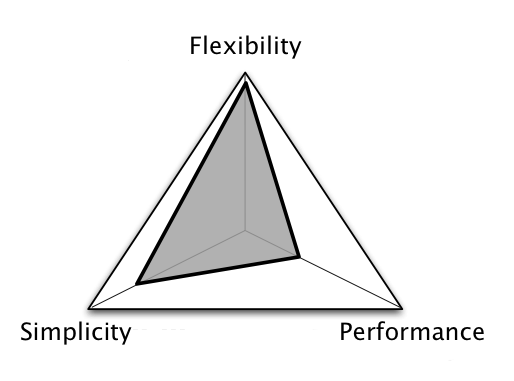
\includegraphics[width=\textwidth]{images/focalpoints}
    \caption{Relative emphasis between three design goals.}
    \label{fig:focalpoints}
\end{figure}

\subsection{Twist's Core Syntax}
\label{sec:syntax}

Twist has a very simple syntax. It has three expression types: 

\begin{enumerate}
	\item Atoms: names, identifiers, and other literals.
	\item Lists: an ordered set of other expressions. 
	\item Calls: a pair of expressions.
\end{enumerate}

This means that every expression in Twist, derived from these three expression types, can be \emph{desugared} to these core elements. The rest of the sections below describes the rest of the syntax.

\subsubsection{Names}
\label{sec:names}

Names are one of the simplest syntactical elements in Twist. They are used for prefix function calls and don't trigger any special parsing. They start with a letter, and don't contain any colons. For example, 

\begin{minted}{java}
what?!, What?!, and WhAt?! 
\end{minted} 

are all the same.

\subsubsection{Operators}
\label{sec:operators}

Operators are a special case in the Twist's syntax. They are parsed like in Io. The Twist's parser intercepts any operator defined by the interpreter, and translate them to method calls. The fact that they do not require explicit parenthesis is convenient. For example, the expression

\begin{minted}{java}
: 1 + 10 * 9 + 1
\end{minted}

is equivalent to

\begin{minted}{java}
: 1 + (10 * (9)) + (1)
\end{minted}

Operators in Twist have a little  bit of operator precedence. Twist has the same operator precedence as with the C language precedence levels.

In addition to these operators, Twist supports three special operators: the braces (\{;\}) operator, the chain (>) operator, and the slash (/>) operator.

The \{;\} is a left-to-right operator. This operator helps express a series of operations that are executed in order. This series of operations, separated by semicolons and surrounded by curly braces, is a syntactical sugar for a ``do'' method call. So this

\begin{minted}{java}
: {display("Hello, World!"); display(1 + 2)}
\end{minted}

is equivalent to

\begin{minted}{java}
: do(display("Hello, World!"); display(1 + 2))
\end{minted}

The > is also a left-to-right operator. This operator helps express nested operations and data flow.  The > operator forms a syntactic glue that binds operations together. For example, the user might think of values passing through a sequence of code transformations---from left to right.

\begin{minted}{java}
: rename-param (
	twitter, facebook) > 
	split > subs ((TS, FS))
\end{minted}

is equivalent to:

\begin{minted}{java}
: subs(split(rename-param(twitter, 
	 facebook)), (TS, FS))
\end{minted}

where:

\begin{enumerate}
	% \item \_ is a placeholder for the output of a previous method call.
	\item The rename command returns the list of results where the parameter ``twitter'' was 
	renamed.
	\item The split command returns the list of functions produced by the split command.
	\item The subs command replaces the TwitterService (abbreviated as TS) type for the 
	FacebookService (FS) type.
\end{enumerate}

The /> operator is similar to the > operator. It differs from the > in the sense of it will attempt to cut down on any failed results, which are a product of the execution of Twist's operations. The following example demonstrates this command. The statement before the : separator is a query. Like this:

\begin{minted}{java}
: factorial +Double => Double : subs(
	(Double, Int)
	 ) /> rename-param(n, nth) 
\end{minted}

Any results, after the application of Twist's /> operator, containing any syntactic or parsing errors will be filtered out from the produced results. Semantic errors will be outside the scope of Twist's functionality. By omitting this operator, developers are willing to see these failed results in the results list.

\subsubsection{Lists}
\label{sec:lists}

A list can be created by separating functions with commas. For example:

\begin{minted}{java}
: 1, 2, 3
\end{minted}

Parentheses are not necessary, but they are often useful since commas have low precedence. For example:

\begin{minted}{java}
: hello a, b     ; means (hello(a), b)
\end{minted}

is different than

\begin{minted}{java}
: hello(a, b)    ; means hello(a, b)
\end{minted}

\subsubsection{Functions}
\label{sec:functions}

In Twist, a name followed by an expression will call that named function and pass it the given argument(s)---if provided. For example:

\begin{minted}{java}
: version (1.0, true)
\end{minted}

This is a function with two arguments. If the version function had zero arguments, then it would look like this:

\begin{minted}{java}
: version
\end{minted}

This function with zero arguments prints the current version of Twist. With two arguments, it prints additional information in regards to Twist's 1.0 version, such as changes that went in version 1.0. 

That's the basic syntax. The Twist parser reads that and then it translates it to the core syntax.

\section{Running Twist}
\label{sec:running}

Twist is also a Web application, and one can access it by using a Web browser. Once opened, the Twist's REPL will start. The command line interface for this interpreter is showed in the Figure~\ref{fig:twist}. 

\subsection{Twist's Interpreter}
\label{sec:interpreter}

A good way to learn Twist is to interact with an interpreter and study its responses. This is very similar to the way people already interact with search engines. For this work, two types of interaction with Twist are considered: 

\begin{enumerate}
	\item Supply an expression, sometimes led by a text search, to be evaluated.
	\item Import a script file with a set of expressions to be evaluated. 
\end{enumerate}	

The following image (Figure~\ref{fig:runtime}) represent the processing of commands issued by a user and handled by Twist:

\begin{figure}[!ht]
    \centering
    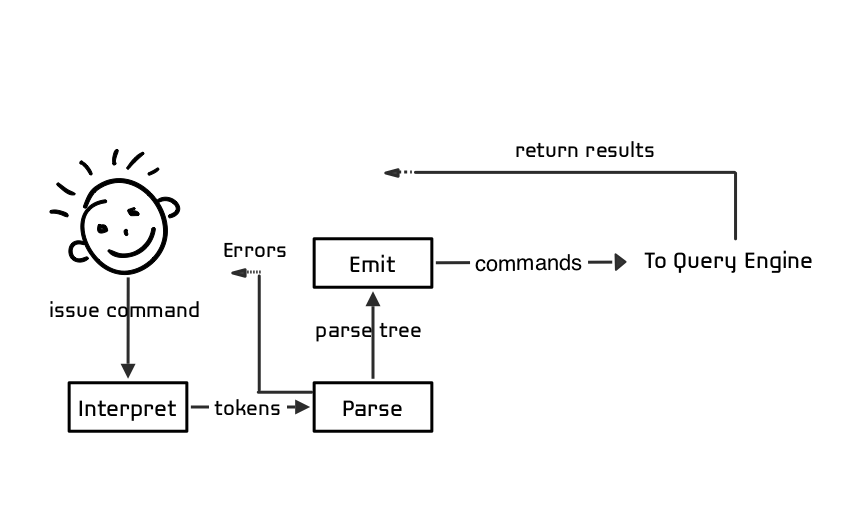
\includegraphics[width=\textwidth]{images/runtime}
    \caption{Twist's runtime processing.}
    \label{fig:runtime}
\end{figure} 

Any errors caused by misusing Twist's syntax and built-in functionality will be displayed to the user right after the user has pressed the enter key. Figure~\ref{fig:error} displays this.

\begin{figure}[!ht]
    \centering
    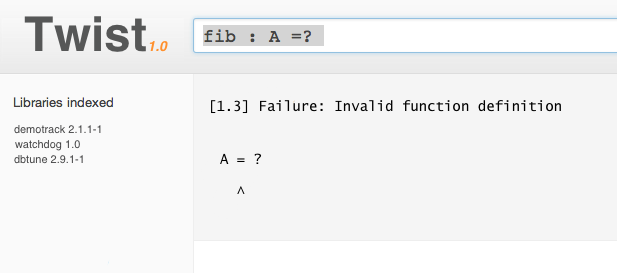
\includegraphics[width=\textwidth]{images/error}
    \caption{Error caused my misusing Twist's syntax and built-in operations.}
    \label{fig:error}
\end{figure}

\subsection{Built-in Functions}
\label{sec:functions}
 
As of now, only a few built-in functions have been designed:

\begin{enumerate}
	\item do <expr>: If the <expr> is anything but a list, Twist will evaluate it and 
	return. If it is a list, then Twist will evaluate each item in the list, in order, 
	and then return the evaluated value.
	
	\item <params> = <body>: It creates an anonymous function. <params> should either be 
	a single name or a list of parameter names. <body> represents the body of a 
	function. It is also an expression. For example, : (a = loc(a) < 20) is an 
	anonymous function that returns true if a snippet's size is less than 20 lines of 
	code. 
	
	\item if(<predicate>, then-clause, else-clause): Twist evaluates the predicate. If 
	the predicate evaluates to true, then it evaluates and returns the <expr>. Otherwise, 
	it will evaluate and return the <expr> in the else clause. For example, : if(true 
	\&\& true, display ``Y'', display ``N'').
	
	\item learn(<name>, <expr>): Twist binds a value to a variable in the current scope. 
	<name> should be a single name. Twist will evaluate <expr> and then it will bound the 
	result to the name. For example, : learn(twist, ``SNIPR's tiny language'' )
   
	\item isbool? <expr>, isint? <expr>, islist? <expr>, isname? <expr>, isunit? <expr>: Twist 
	evaluates <expr>, and then returns true if the result is the given type.
 	
	\item <int> <expr>: Twist evaluates <expr>, expecting to be a list. Then, it will 
	return the item at the <int> position in the list. For example, : 2 (1, 2, 3) will 
	return 3.
	
	\item size <expr>: Twist evaluates <expr>, expecting it to be a list. Then, it will 
	return the size of the list.
\end{enumerate}

\subsection{Built-in Commands}
\label{sec:retargetingops}

Only a few built-in commands are designed:

\begin{enumerate}
	\item import <url>: The command will import a twist file containing a set of 
	user-defined functions. Once the twist file is loaded, any function in the file will 
	be interpreted by the Twist's interpreter and ready to be used by the user.
	
	\item list: It returns the current list of results, or () if it is empty.
	
	\item select(<list>, <predicate>): It applies the <predicate>(usually an anonymous function) 
	to the given list of results. When using the current list of results (results produced by a 
	query) or using the > or /> operators, the list is implicit in the operation. Therefore it can 
	be omitted. For example, fibonacci +Int=>Int : select(loc > 20), which is the same as 
	fibonacci +Int=>Int : select(list, a = loc(a) > 20). Or, fibonacci +Int=>Int : select(loc > 
	20) > select(loc < 7).
	
	\item apply(<list>, <operation>): It applies an <operation>(e.g., a retargeting operation) 
	to the given list of results. Similar to the select operation, the list of results can be 
	omitted. For example, fibonacci +Int=>Int : apply(rename-method(from, to)). Or, fibonacci 
	+Int=>Int : apply(rename-method\footnote{learn(rename-method, a, b, name(method(a), b))}(from, 
	to)) > apply(rename-param\footnote{learn(rename-param, a, b, name(param(a), b))}(from, to)).
		
	\item reject(<list>, <predicate>): It is similar to the select operation. The main difference 
	is that instead of selecting those results that matched the predicate, it will reject those 
	ones who do. 
	
	\item undo, redo: The undo command rolls back a change made to one or more results. 
	The redo is the opposite to the undo command.  
	
	\item loc(<result>): It returns the size of snippet (represented as a result in the 
	list of results produced by a query). When using this operation within the select and reject 
	operations, the <result> is implicit in the operation; therefore it can be omitted. 
	
	\item morph(<list>, <pairs-of-statements>): It tries to change from one type of statement 
	(e.g., switch statement) to another type (e.g., a series of if:else statements). Returning an 
	error if the change cannot be made. Similar to the select, apply, and reject operations, the 
	list of results can be omitted (this is the same for the rest of operations). For example, : 
	morph((if:else, switch)) (Figure~\ref{fig:basealternative} shows such a transformation).  
	
	\item err(result): It returns true if the result contains syntactic (parsing) errors. 
	It returns false otherwise. Similar to the loc operation, when used in the select and reject 
	operations, the <result> can be omitted.
	
	\item subs(<list>, <pairs-of-types>). It replaces one type for another. The 
	<pairs-of-types> is a list of source-target pairs. For example, : subs((Int, Double),
	(ArrayList, LinkedList)).
	
	\item split(<list>, <int> = 2): It splits a method into <int> parts. Returning an 
	error if the change cannot be made. If <int> is not specified, the it is assumed that the user 
	wants to split the method into two methods. For example, fibonacci +Int=>Int : split

   \item merge(<list>, <list-of-methods>, <method>): This is the opposite of the split command. 
	For example, fibonacci +Int=>Int : merge((method(fib\_helper), method(fib)))
	
	\item param <name>, method <name>: It returns either a param matching a given name, 
	or a method matching a given name.
	
	\item name (<member>, <new-name>): It gives a new name to an existing member (parameter in 
	a method, or the name of the method).
	
\end{enumerate}

\subsection{Mixing Queries and Commands}
\label{sec:queriescommands}

Code searches can be either textual (a list of words), or by type (type signature\footnote{<InputTypes>=><OutputType>}), or both. A search is considered a text search unless it contains a combination of text and symbols, or if starts with `:'. To search for both a type signature and a name, place the + symbol between them. Any expression written after the : symbol represents a command to be executed against the results of a query. A few examples are illustrated below:

\begin{minted}{java}
// search for the text fibonacci	
fibonacci
// search for text factorial and the 
// text fibonacci
factorial fibonacci
// search for the text fibonacci, with 
// the type signature Int=>BigInteger 
fibonacci +Int=>BigInteger 
// gives a name to the first item in the 
// current list of results.
: learn(first, 0 (list))
// rename the first item's parameter 
// from n to number.
fibonacci +Int=>Int : first > 
rename-param(n, number) 
\end{minted}
	 
Let's make one important observation. The + symbol, besides helping search by type, can be used to reduce the search scope of a query. For example, if one knows in advance what library (separated by comma if there are more than one library) to search, then one can use the + (it means ``only in'') to specify the name of the library. Like this:

\begin{minted}{java}
: fibonacci +supermath-1.0 
\end{minted}

The opposite of + symbol is the - symbol. This symbol means ``everywhere except in.'' The following example illustrates this behavior.

\begin{minted}{java}
: fibonacci +like-1.0 -dontlike-1.0
\end{minted}
 
 
This chapter has introduced Twist, a language for interacting with search results, and combining and executing code retargeting operations. 
